\subsection{MTU}

Máximo tamaño de paquete de datos que se puede transferir en IP. Depende de la capa de enlace, por lo que no se tiene la misma MTU en Ethernet que en Wi-Fi. El problema surge cuando se quieren enviar paquetes cuyo tamaño es mayor al MTU.

$$ \mathrm{MTU} = \mathrm{MSS} + \mathrm{IP}_{\mathrm{header}} + \mathrm{TCP}_{\mathrm{header}} $$

Para solucionarlo, se fragmenta el datagrama en partes, donde cada fragmento se transmite en un paquete IP diferente. El proceso de fragmentación puede darse tanto en hosts como en routers. Sin embargo, el ensamble solo se realiza en el destino. IP es sin conexion, lo paquetes son tratados individualmente. La informacion para el ensamblado viaja en el header de IP: fragment offset y flags. No pueden llegar sin ensamblar a TCP/UDP. En caso de que uno o más no lleguen, se descarta toda la secuencia.

Los flags pueden ser tres:

\begin{itemize}
    \item [X]: reservado, no se usa
    \item [D]: Do no fragment. Indica si se puede fragmentar o no
    \item [M]: More Fragments. Indica si es el ultimo fragmento o hay más
\end{itemize}

El fragment Offset tiene 3 bits menos que el Total Lenght debido a los flags. Además, cuenta en unidades de 8 bytes. De esta manera, cada bit que nos movemos en el fragment offset implica moverse 8 bits en el total lenght

\begin{center}
    \begin{tabular}{c|c|c|c}
    \hline
         X(1) & D(1) & M(1) & Fragment offset (13)  \\
    \hline     
    \end{tabular}
\end{center}

\textbf{Ejemplo} \\

Suponiendo $ \mathrm{MTU} = 550 B = 530 B_{\mathrm{payload}} + 20 B_{\mathrm{header}} $

Se quiere envian un payload de 800 B. El máximo payload a enviar por paquete es 530. Entonces será un paquete de 530 bytes y otro de 270 bytes.

$$\mathrm{Fragmento}_1 = 530 B$$
$$\mathrm{Fragmento}_2 = 270 B$$

Calculemos el fragment offset de cada uno.

$$ \mathrm{FragmenOffset}_1 = 0 $$
$$ \mathrm{FragmenOffset}_2 =  ? $$

\begin{center}
    \begin{tabular}{c|c}
        Offset Real & Fragment Offset \\
        \hline
        \hline
        8 Bytes & 1 \\
        \hline
        530 Bytes & \textbf{66.25}
    \end{tabular}
\end{center}

66.25 no puede ser expresado en número binario, por lo que hay que cambiar el tamaño de los fragmentos. Para calcular el nuevo tamaño se usa la siguiente fórmula:

$$ \mathrm{FragmentPayloadSize} = \mathrm{floor}(\frac{\mathrm{MaxPayloadSize}}{8}) \cdot 8 $$

En nuestro caso $\mathrm{floor}(\frac{\mathrm{530 B}}{8}) \cdot 8 = 528 B$

$$\mathrm{Fragmento}_1 = 528 B$$
$$\mathrm{Fragmento}_2 = 272 B$$

\begin{center}
    \begin{tabular}{c|c}
        Offset Real & Fragment Offset \\
        \hline
        \hline
        8 Bytes & 1 \\
        \hline
        528 Bytes & \textbf{66}
    \end{tabular}
\end{center}


\subsection{Ejercicio de Parcial}

\subsubsection{Ejercicio 1}
El host A quiere enviar un paquete de tamaño total 620 bytes al host B. El valor del flag Do not fragment es cero.

\begin{figure}[H]
\centering
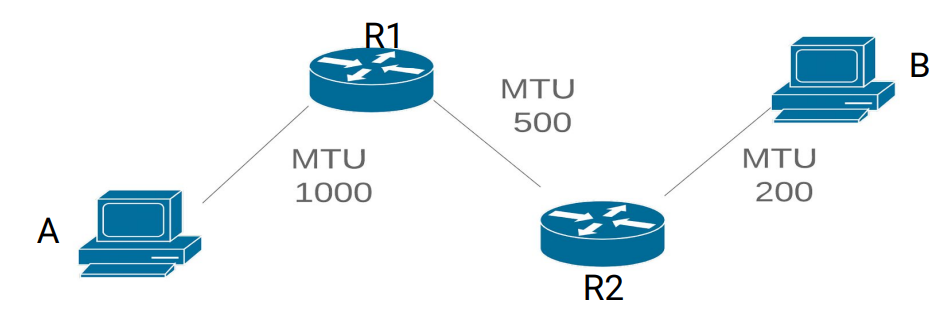
\includegraphics[width=\textwidth]{imagenes/frag1.png}
\end{figure}

\textbf{A - R1}\\
En la conexion del host a con R1 se comprueba que el MTU es mayor al paquete que desea envíar. Por lo que se envia el paquete sin fragmentacion

$$ \mathrm{MTU} = 1000 $$
$$ \mathrm{Paquete} = 620 $$
$$ \mathrm{MTU}  \geq \mathrm{Paquete}$$

\begin{itemize}
    \item Total Lenght: 620 bytes
    \item X: reservado
    \item D: 0
    \item M: 0
    \item Fragment Offset: 0
\end{itemize}


\textbf{R1 - R2}\\

En la conexión de R1 con R2 se verifica que el MTU es menor a el paquete a enviar, además el Do Not Fragment es cero por lo que debe fragmentarse el paquete.

$$ \mathrm{MTU} = 500 $$
$$ \mathrm{Paquete} = 620 $$
$$ \mathrm{MTU}  \le \mathrm{Paquete}$$

El MTU incluye al header, asumo que es de 20 Bytes. Entonces en máximo tamaño de payload será de 480 Bytes

$$ \mathrm{MaxPayloadSize} = \mathrm{MTU} - \mathrm{Lenght}(\mathrm{Header}) = 500 - 20 = 480 $$

$$\mathrm{floor}(\frac{\mathrm{480 B}}{8}) \cdot 8 = 480 B$$

De esta manera se van a enviar 2 fragmentos:

\textbf{Recordar no tener en cuenta el header del mensaje original.}


$$ \mathrm{PayloadOriginal} = 620 - 20 = 600 $$
$$\mathrm{Fragmento}_1 = 480 B$$
\begin{itemize}
    \item Total Lenght: 480 + 20 bytes
    \item X: reservado
    \item D: 0
    \item M: 1
    \item Fragment Offset: 0
\end{itemize}

$$\mathrm{Fragmento}_2 = 600 - 480 = 120 B$$

\begin{center}
    \begin{tabular}{c|c}
        Offset Real & Fragment Offset \\
        \hline
        \hline
        8 Bytes & 1 \\
        \hline
        480 Bytes & \textbf{60}
    \end{tabular}
\end{center}

\begin{itemize}
    \item Total Lenght: 120 + 20 bytes
    \item X: reservado
    \item D: 0
    \item M: 0
    \item Fragment Offset: 60
\end{itemize}


\textbf{R2 - RB}\\

Para el primer fragmento, el MTU es menor al tamaño, por lo que habrá que fragmentar. El Largo total del segundo fragmento puede reenviarse sin fragmentar.


$$ \mathrm{MTU} = 200 $$
$$ \mathrm{Fragmento}_1 = 500 $$

$$ \mathrm{MaxPayloadSize} = \mathrm{MTU} - \mathrm{Lenght}(\mathrm{Header}) = 200 - 20 = 180 $$

$$ \mathrm{FragmentPayloadSize} = \mathrm{floor}(\frac{\mathrm{MaxPayloadSize}}{8}) \cdot 8 = \mathrm{floor}(\frac{\mathrm{180}}{8}) \cdot 8  = 176 $$

Recordar de que el payload del fragmento 1 es de 480. Entonces se enviarán dos fragmentos de 176 y uno de 128

\begin{center}
    \begin{tabular}{c|c}
        Offset Real & Fragment Offset \\
        \hline
        \hline
        8 Bytes & 1 \\
        \hline
        176 Bytes & \textbf{22} \\
        \hline
        352 Bytes & \textbf{44}
    \end{tabular}
\end{center}

\begin{center}
    \begin{tabular}{c|c|c|c|c|c}
    Fragmento & Total Lenght & X & D & M & Fragment Offset \\
        \hline
        \hline
    $ \mathrm{Fragmento}_{1_1} $  &  176 + 20  & X & 0 & 1 & 0   \\
    \hline
    $ \mathrm{Fragmento}_{1_2} $  &  176 + 20  & X & 0 & 1 & 22 \\
    \hline
    $ \mathrm{Fragmento}_{1_3} $ &  128 + 20  & X & 0 & 1 & 44 \\
    \hline
    $ \mathrm{Fragmento}_{2} $  & 120 + 20 & X & 0 & 0 & 60
    \end{tabular}
\end{center}

La suma de los payloads, da un payload total de 600 que es el payload que se tenia originalmente (más 20 de header)

\subsubsection{Ejercicio 2}


El host A envia un datagrama IP cuyo payload es 1480 Bytes.

\begin{figure}[H]
\centering

\includegraphics[width=\textwidth]{imagenes/enunciadoFragmentacion.png}
\end{figure}


El paquete es de 1500 bytes (1480 + 20 del header). En el primer traspaso, alcanza el MTU.

$$ \mathrm{MaxPayloadSize} = MTU - \mathrm{Lenght}(\mathrm{Header}) = 1500 - 20 = 1480 $$
$$\mathrm{floor}(\frac{\mathrm{1480 B}}{8}) \cdot 8 = 185 B$$

No es necesario fragmentar en este primer tramo.

En el tramo del primer al segundo router hay que fragmentar, ya que el MTU es menor al tamaño del paquete. Se calcula el máximo payload para este tramo:

$$ \mathrm{MaxPayloadSize} = MTU - \mathrm{Lenght}(\mathrm{Header}) = 532 - 20 = 502 $$

$$\mathrm{floor}(\frac{\mathrm{502 B}}{8}) \cdot 8 = 496 B$$

\begin{center}
    \begin{tabular}{c|c|c|c}
        Fragmento & Total Lenght & Fragment Offset & More Fragments \\
        \hline
        \hline
        $ \mathrm{Fragmento}_1 $ & 496 + 20  & 0 & 1\\
        $ \mathrm{Fragmento}_2 $ &  496 + 20 & 62 & 1\\
        $ \mathrm{Fragmento}_3 $ & 488 + 20 & 124 & 0\\
    \end{tabular}
\end{center}

Para el tramo del segunto router al Host B habrá que fragmentar todos ya que el MTU es más chico.

$$ \mathrm{MaxPayloadSize} = MTU - \mathrm{Lenght}(\mathrm{Header}) = 186 - 20 = 166 $$

$$\mathrm{floor}(\frac{\mathrm{166 B}}{8}) \cdot 8 = 160 B$$



\begin{center}
    \begin{tabular}{c|c|c|c}
        Fragmento & Total Lenght & Fragment Offset & More Fragments \\
        \hline
        \hline
        $ \mathrm{Fragmento}_{11} $ & 160 + 20  & 0 & 1\\
        \hline
        $ \mathrm{Fragmento}_{12} $ & 160 + 20  & 20 & 1\\
        \hline
        $ \mathrm{Fragmento}_{13} $ & 160 + 20  & 40 & 1\\
        \hline
        $ \mathrm{Fragmento}_{14} $ & 16 + 20  & 60 & 1\\
        \hline
        \hline
        \hline
        $ \mathrm{Fragmento}_{21} $ & 160 + 20  & 62 & 1\\
        \hline
        $ \mathrm{Fragmento}_{22} $ & 160 + 20  & 82 & 1\\
        \hline
        $ \mathrm{Fragmento}_{23} $ & 160 + 20  & 102 & 1\\
        \hline
        $ \mathrm{Fragmento}_{24} $ & 16 + 20  & 122 & 1\\
        \hline
        \hline
        \hline
        $ \mathrm{Fragmento}_{31} $ & 160 + 20  & 124 & 1\\
        \hline
        $ \mathrm{Fragmento}_{32} $ & 160 + 20  & 144 & 1\\
        \hline
        $ \mathrm{Fragmento}_{33} $ & 160 + 20  & 164 & 1\\
        \hline
        $ \mathrm{Fragmento}_{34} $ & 8 + 20  & 184 & 0\\
    \end{tabular}
\end{center}

Se puede verificar ya que el fragment offset total de la segunda tabla es $124 + \frac{488}{8} = 185$ y el fragment offset total de la última tabla es $184 + \frac{8}{8} = 185$. 
Además si se suman los payloads se llega a un total de 1480, igual al payload del mensaje original.


